

\documentclass[10pt,dvipsnames]{beamer}

%\usepackage{pgfpages}
%\mode<handout>{\setbeamercolor{background canvas}{bg=black!20}}
%\pgfpagesuselayout{4 on 1}[letterpaper,border shrink=5mm]

\usepackage{lmodern}
\usepackage{xcolor}
\usepackage[utf8]{inputenc}
\usepackage{amsmath, amsfonts}
\usepackage{verbatim}
\usepackage{tikz}
\usetikzlibrary{decorations.pathreplacing}
\beamertemplatenavigationsymbolsempty
\setbeamertemplate{footline}[frame number]
\addtolength{\oddsidemargin}{-3pt}

\definecolor{dgreen}{rgb}{0.,0.6,0.}
\definecolor{highlight}{rgb}{0.,0.6,0.}

\usepackage{multimedia}

\title{Cancer classification based on miRNA profiles using ASP} 
\author{K. Becker and H. Klarner}
\date{Berlin, Mai 2016}
\institute{
Freie Universität Berlin, Germany
}
% logo of my university
\titlegraphic{\vfill
\includegraphics[width=2cm]{FU-Logo}\hspace*{4.75cm}~%
   
\includegraphics[width=2cm]{BMBF-Logo}
}

\begin{document}


\frame{\titlepage}


%{\tiny R. Thomas. "Regulatory networks seen as asynchronous automata." JTB, 1991}


\begin{frame}{Selective cell targeting}
\large
\begin{itemize}
\item \textbf{Problem:} Discrimination of tumor from healthy tissues
\end{itemize}

\vspace{0.5cm}
\begin{center}
\only<1>{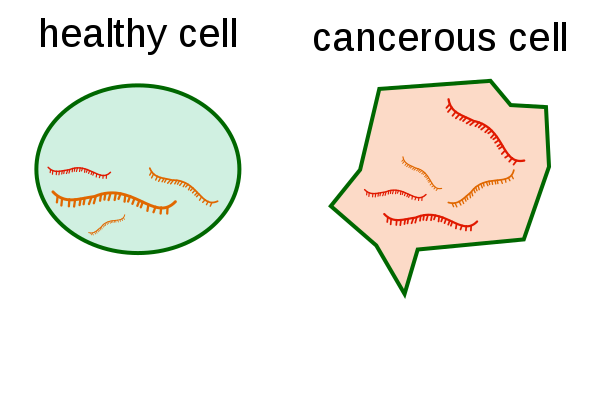
\includegraphics[scale=0.25]{cells.png}}
\only<2>{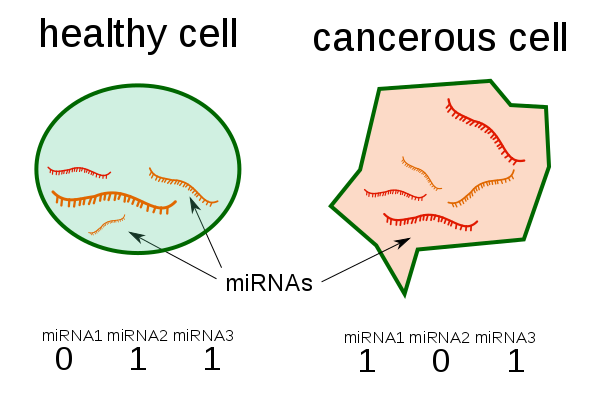
\includegraphics[scale=0.25]{cells1.png}}
\end{center}
\vspace{0.5cm}

\begin{itemize}
\item<2> \textbf{Idea:} Cells differ in miRNA profiles
\end{itemize}
\end{frame}


\begin{frame}{In vitro classification}
\end{frame}


\begin{frame}{Constraints from biology}
\begin{itemize}
\item less than 10 inputs in total
\item no more than 6 inputs attached to the AND gate
\item no more than 3 inputs atttached to any OR gate
\item no NOT gates attached to an OR gate
\item no more than 2 OR gates
\item no more than 4 NOT gates
\end{itemize}
\end{frame}


\begin{frame}[fragile]{Input: Data}
\begin{center}
\begin{tabular}{|c|c|c|c|c|}
\hline
ID&	Annots&	g1&	g2&	g3\\
\hline
1&	0&	1&	1&	0\\
2&	0&	0&	0&	1\\
3&	1&	0&	1&	0\\
\hline
\end{tabular}
\begin{tikzpicture}[overlay]
\draw[decorate, decoration={brace}]
      (-2.2,1.2) -- node[above=0.15cm, scale=1] {\textbf{miRNAs}} (-0.2,1.2);
\draw[decorate, decoration={brace}]
      (-3.8,1.2) -- node[above=0.15cm, scale=1] {\textbf{cancer?}} (-2.5,1.2);
\draw[decorate, decoration={brace}]
      (-5,-0.7) -- node[left=0.15cm, scale=1] {\textbf{tissues}} (-5,0.5);
\end{tikzpicture}
\end{center}
\vspace{0.2cm}
\begin{verbatim}
tissue(1,healthy). tissue(2,healthy). tissue(3,cancer).
 
data(1,g1,high). data(1,g2,high). data(1,g3,low).
data(2,g1,low).  data(2,g2,low).  data(2,g3,high).
data(3,g1,low).  data(3,g2,high). data(3,g3,low).
 
is_mirna(Y) :- data(X,Y,Z).
\end{verbatim}
\end{frame}



\begin{frame}[fragile]{Input: Classifier structure}
\begin{center}
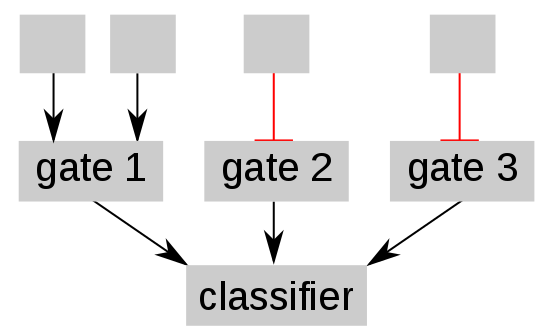
\includegraphics[scale=0.25]{classifier.png}
\end{center}
\vspace{0.3cm}

\begin{verbatim}
is_gate_type(type1).

upper_bound_pos_inputs(type1, 1). 
upper_bound_neg_inputs(type1, 0). 
lower_bound_pos_inputs(type1, 0). 
lower_bound_neg_inputs(type1, 0). 
upper_bound_gate_occurence(type1, 1). 
 
upper_bound_inputs(2).
\end{verbatim}

%\begin{tikzpicture}[overlay]
%\draw[decorate, decoration={brace}]
%      (6,3.35) -- node[right=0.15cm, scale=1] {\textbf{bounds for gate type 1}} (6,1.35);
%\end{tikzpicture}
\end{frame}


\begin{frame}[fragile]{Decision 1: Number of gates}
\small
\begin{verbatim}
1 {number_of_gates(1..2)} 1.

is_integer(1..2).
is_gate_id(GateID) :- number_of_gates(X),is_integer(GateID), 
                      GateID<=X.
\end{verbatim}
\end{frame}


\begin{frame}[fragile]{Decision 2: Gate types}
\small
\begin{verbatim}
1 {gate_type(GateID, X) : is_gate_type(X)} 1 :- is_gate_id(GateID).
\end{verbatim}
\end{frame}


\begin{frame}[fragile]{Decision 3: Inputs for each gate}
\small
{\color{blue}{\large positive inputs:}}
\begin{verbatim}
X{gate_input(GateID,positive,MiRNA):is_mirna(MiRNA)}Y 
   :-is_gate_id(GateID),gate_type(GateID,GateType),
     lower_bound_pos_inputs(GateType,X), 
     upper_bound_pos_inputs(GateType,Y).
\end{verbatim}

{\color{blue}{\large negative inputs:}}
\begin{verbatim}
X{gate_input(GateID,negative,MiRNA):is_mirna(MiRNA)}Y 
   :-is_gate_id(GateID),gate_type(GateID,GateType),
     lower_bound_neg_inputs(GateType,X),
     upper_bound_neg_inputs(GateType,Y).
\end{verbatim}
\end{frame}



\begin{frame}[fragile]{Constraints}
 \begin{itemize}
  \item conditional count constraints
  \item
 \end{itemize}

\end{frame}


\begin{frame}[fragile]{Gates must have inputs}
 \texttt{1 \{gate\_input(GateID, Sign, MiRNA):}
 \begin{verbatim}
  1 {gate_input(GateID, Sign, MiRNA):
     is_sign(Sign), is_mirna(MiRNA)} :- is_gate_id(GateID).
 \end{verbatim}
\end{frame}


\begin{frame}[fragile]{Inputs must be unique}
 \begin{verbatim}
  {gate_input(GateID,Sign,MiRNA):
    is_sign(Sign), is_gate(GateID)} 1 :- is_mirna(MiRNA).
 \end{verbatim}
\end{frame}


\begin{frame}[fragile]{Number of inputs is bounded}
 \begin{verbatim}
  {gate_input(GateID, Sign, MiRNA):
    is_gate_id(GateID), is_sign(Sign), is_mirna(MiRNA)} X :-
  upper_bound_inputs(X).
 \end{verbatim}
\end{frame}

\begin{frame}[fragile]{Occurences of gates}
 \begin{verbatim}
  {gate_type(GateID,GateType):
     is_gate_type(GateType),
     is_gate_id(GateID)} X :-
    upper_bound_gate_occurence(GateType,X).
 \end{verbatim}
\end{frame}
 

\begin{frame}[fragile]{Activity of gates}
 \begin{verbatim}
 gate_fires(GateID,TissueID) :-
   gate_input(GateID,positive,MiRNA),
   data(TissueID,MiRNA,high).
   
 gate_fires(GateID,TissueID) :-
   gate_input(GateID,negative,MiRNA),
   data(TissueID,MiRNA,low).
 \end{verbatim}
\end{frame}

\begin{frame}[fragile]{The classifier}
 \begin{verbatim}
  classifier(TissueID, healthy) :-
    not gate_fires(GateID, TissueID),
    is_gate_id(GateID), is_tissue_id(TissueID).
    
  classifier(TissueID, cancer) :-
    not classifier(TissueID, healthy),
    is_tissue_id(TissueID).
 \end{verbatim}
\end{frame}



\begin{frame}{Optimization}
 \begin{itemize}
  \item single objective
  \item with priorities
  \item weighted sum
 \end{itemize}
\end{frame}

\begin{frame}[fragile]{Single Objective}
 \begin{verbatim}
  #minimize{ 1@1,GateID:gate_input(GateID,Sign,MiRNA) }.
  #minimize{ 1@2,MiRNA: gate_input(GateID,Sign,MiRNA) }.
 \end{verbatim}
\end{frame}

\begin{frame}[fragile]{Priorities}
 \begin{verbatim}
  #minimize{ 1@1,GateID:gate_input(GateID,Sign,MiRNA) }.
  #minimize{ 1@2,MiRNA: gate_input(GateID,Sign,MiRNA) }.
 \end{verbatim}
\end{frame}


\end{document}

 